\documentclass[11pt]{article}
\usepackage{listings}

% Use wide margins, but not quite so wide as fullpage.sty
\marginparwidth 0.5in 
\oddsidemargin 0.25in 
\evensidemargin 0.25in 
\marginparsep 0.25in
\topmargin 0.25in 
\textwidth 6in \textheight 8 in
% That's about enough definitions
\usepackage{hyperref}
% multirow allows you to combine rows in columns
\usepackage{multirow}
% tabularx allows manual tweaking of column width
\usepackage{tabularx}
% longtable does better format for tables that span pages
\usepackage{longtable}
\documentclass{article}
\usepackage{graphicx}
\begin{document}
% this is an alternate method of creating a title
%\hfill\vbox{\hbox{Gius, Mark}
%       \hbox{Cpe 456, Section 01}  
%       \hbox{Lab 1}    
%       \hbox{\today}}\par
%
%\bigskip
%\centerline{\Large\bf Lab 1: Security Audit}\par
%\bigskip
\author{Daniel Ocampo \& Moses Alcantraz}
\title{Lab 7: Psychological analysis  Exploratory Data Analysis}
\maketitle

\section{Objective}
To explore statistical tools which are relevant for the evaluation of psychological data. In particular,
to be able to research how to use new R-statistics software packages and apply them to particular
contexts for which they were designed. To extract knowledge from the produced visualizations and
extracted interpretation of results.


\section{Part One: Obtain your data:}

Obtain your data: You may obtain your data from any online source as long as it is a
credible source and that the data stems from the psychology discipline. For an idea, you could
select the data available by the Cornell University website: https://www.ciser.cornell.
edu/ASPs/datasource.asp.


The data that I was able to find was from the Labor bureau statistics \href{https://www.bls.gov/cex/csxstnd.htm#2010}{BLS}.\\ The reason I chose this data set was because of the wealth effects, I want to see based on the data if that is real. How much impact the financial crisis of 2008 has done to impact  the economy. 





\section{Part Two: Description of Data}

You are to write a short report to describe your data. Discuss what
the data contains and its purpose (i.e., why was this data collected, for what purpose?). You
may need to look this information up online from sources other than the one where you found
it.



I found this data based on the simple fact that is has so much information. One of thing that I find interesting  is how people spend their money. according to Hayek an economist people make rational decisions. The data wide range of data  from consumer spending. The U.S currently has about a 1.5\% percent GDP growth. The U.S has one of the strongest economies, and therefore I would like to see how the great economy works. If US has a good GDP which is a measurment of the health of an economy.  The data From \href{https://www.bls.gov/cex/csxstnd.htm#2010}{BLS} has Tons of data from Consumer Spending.  The data contains things such as products us consumers were spending on. I feel one of the most important things Americans should spend on is Health, because in the long run  medical cost can ruin a person lives causing them to spend less, which intern is bad for the econmy considering the fact that most our GDP is based on consumer Spending. 



\section{part three:Tools and Software}

Using your credible data, you are to use the psych package to perform a
correlation analysis over variables that you will study in connection to your research questions.


\begin{lstlisting}[language=R]

install.packages("gapminder")
install.packages("dslabs")
install.packages("dplyr")
install.packages("tidyverse")
install.packages("psych")
library(gapminder)
library(dplyr)
library(tidyverse)
library(ggplot2)
library(psych)

library(ctv)
task.views("Psychometrics")


#rm(gapminder)

#CSUS2011 <- read.clipboard.tab()
#CSUS2011 <-food
CSAvg <- read.csv(file = "/home/o/ocampod/fall2017/cs390-ochampoo/Data-Analytics/lab7/ConsumerSpending/lab7DataFixCol.csv", header=TRUE, sep= ",")


#### Pysch tutorial ###
boxplot(annualExpend ~ Age)
describe(CSAvg)
headTail(CSAvg)

pairs.panels(CSAvg)

outlier(CSAvg)

cleaned <- scrub(CSAvg, max=9)
error.bars(CSAvg)
View(CSAvg)
RandomData <- select(CSAvg, IncomeAfterTax,annualExpend,IncomeBeforeTax,HealthcareSpending)
View(RandomData)
lowerCor(RandomData)
View(income)
corPlot(RandomData)
corr.test(RandomData)

fa.parallel(RandomData)
vss(RandomData)
fa(RandomData)
iclust(RandomData)
omega(RandomData)
principal(RandomData)
CSAvg[1,]

CSyear00 <- filter(
  CSAvg ,
  Year  ==  2000
  )

View(CSyear00)

###########################Liner Regressions Question 1################################ 
## Do young people spend more on in 10 years? 

ages25 <- filter(
  
  CSAvg,
    Age == "Under 25 years"  )

View(ages25)
qplot(Year, AlcoholicSpending, data = ages25, alpha = I(1/4)) + geom_smooth(method = lm, se = F)
ggsave("/home/o/ocampod/fall2017/cs390-ochampoo/Data-Analytics/lab7/quest1.png")
### It turns out that the data tells me that they consume less during expected ecpnomic downfalls. 
#populationdata <- gapminder

#year07 <- filter(
 # gapminder ,
 #year ==  2007 
  
#)
######## Question 2 ####################
# the Tech bubble occured in 2001
# health insurance among older people change? 
### Based on what I see health insurance has always gone up and does not 
#seem to slow down of older people, seems to be where all of money is spent.  

Healthinsurance <- filter(
  
  CSAvg,Age == "65 years and older" )
View(Healthinsurance)


qplot(Year, HealthcareSpending, data = 
Healthinsurance, alpha = I(1/4)) 
+ geom_smooth(method = lm, se = F)
ggsave
("/home/o/ocampod/fall2017
/cs390-ochampoo/Data-Analytics/lab7/quest2.png")
##################Test######
#### ?   
HealthCor <- select(CSAvg,Year,HealthcareSpending)
View(HealthCor)
corr.test(HealthCor, method = "pearson")
mean(HealthCor, na.rm = T)
plot(HealthCor)
#ttest <- tibble::tribble( ~Observation, ~Colour, ~percentFull, 1,"Green", 70,
 #                               2,"Purple",30,
#                                3,"Green",50,
 #                               4,"Purple",20,
  #                              5,"Purple",15,
   #                             6,"Green",90,
    #                            7,"Purple",40,
     #                           8,"Green",60,
      #                          9,"Purple",15)#

#data_drinks <- data_drinks %>% select(Colour, percentFull)
#Run the t-test: a comparison of means.
#t.test(data = ttest,  ~ Colour) these are just test from previous class codes 

##### Question 3
#### How much of diffrence is 2000 from 2002? (The tech bubble )


twoData <- filter(HealthCor, Year == 2000 | Year == 2002)
View(twoData)
t.test(data = twoData,  HealthcareSpending ~ Year)
#t.test(data = HealthCor,  HealthcareSpending ~ Year)


#CSAvg\$annualExpend
<- factor(c(rep("wages", dim(wages)[1]), rep("pWages", dim(pWages)[1])))
#ggplot(CSAvg, aes(x=HealthcareSpending, y=annualExpend, col = dataset, shape = dataset)) 
+ geom_point(alpha = I(1/4)) + geom_smooth( method = lm)






# Question 4 ###
### What is the difference in annual expenditure between 2008 and 2009?
#We must note that there was a real estate crisis going on during that time. 
#### average difference between was not a lot but there is less spent in 2009 according to the T.test data. 
housingCrisis <- select(CSAvg, annualExpend,Year)
housingCrisis <- filter(housingCrisis, Year == 2008 | Year == 2009) 
View(housingCrisis)

t.test(data = housingCrisis,  annualExpend ~ Year)
 
# question 5 #
### How much has annual spending changed throughout the years?
View(CSAvg)
ggplot(data = CSAvg) +
  geom_point(mapping = aes(x = Year, y = annualExpend, color = Age))
ggsave("/home/o/ocampod/fall2017/cs390-ochampoo/Data-Analytics/lab7/quest5.png")



## I see that certain age groups tend to buy more things, even though there are is 
huge market for the baby boomers usally people in their late 30s and early 40 tend to spend the most
### if I would want to start a bussiness I would want to get that markets. 




##### This was my first Idea, but is not going to be used but still good code for future refrence
gdp07 <- select(year07,gdpPercap)
View(gdp07)
gdp07 <- rename(gdp07,gdpPercap07 = gdpPercap)

View(gdp07)
  
year06 <- filter(
  gapminder ,
  year ==  2006
  
)  
#rm(gdpbByyears)   

year05 <- filter(
  populationdata ,
  year ==  2005
  
)







#gapminder <- mutate( gapminder, avg = mean(gdpPercap,gdppercap))

write.csv(MyData, file = "MyData.csv")



\end{lstlisting}




\section{Part Four:Answerable Questions}


These are some of the first question that I came up with while doing my research in about consumer spending, the question are answered on the source code (Section 4).  
\begin{itemize}
\item Do young  people  spend more on in  10  years ?
\item How much alcohol are young people consuming throughout the years? 
\item health insurance among older people change?  
\item  What was the average total expenditure between 2008 and 2009?
\item What age group spends the most amount of Money?
\end{itemize}

\begin{figure}[h]
\caption{How much alcohol are young people consuming throughout the years?}
\centering
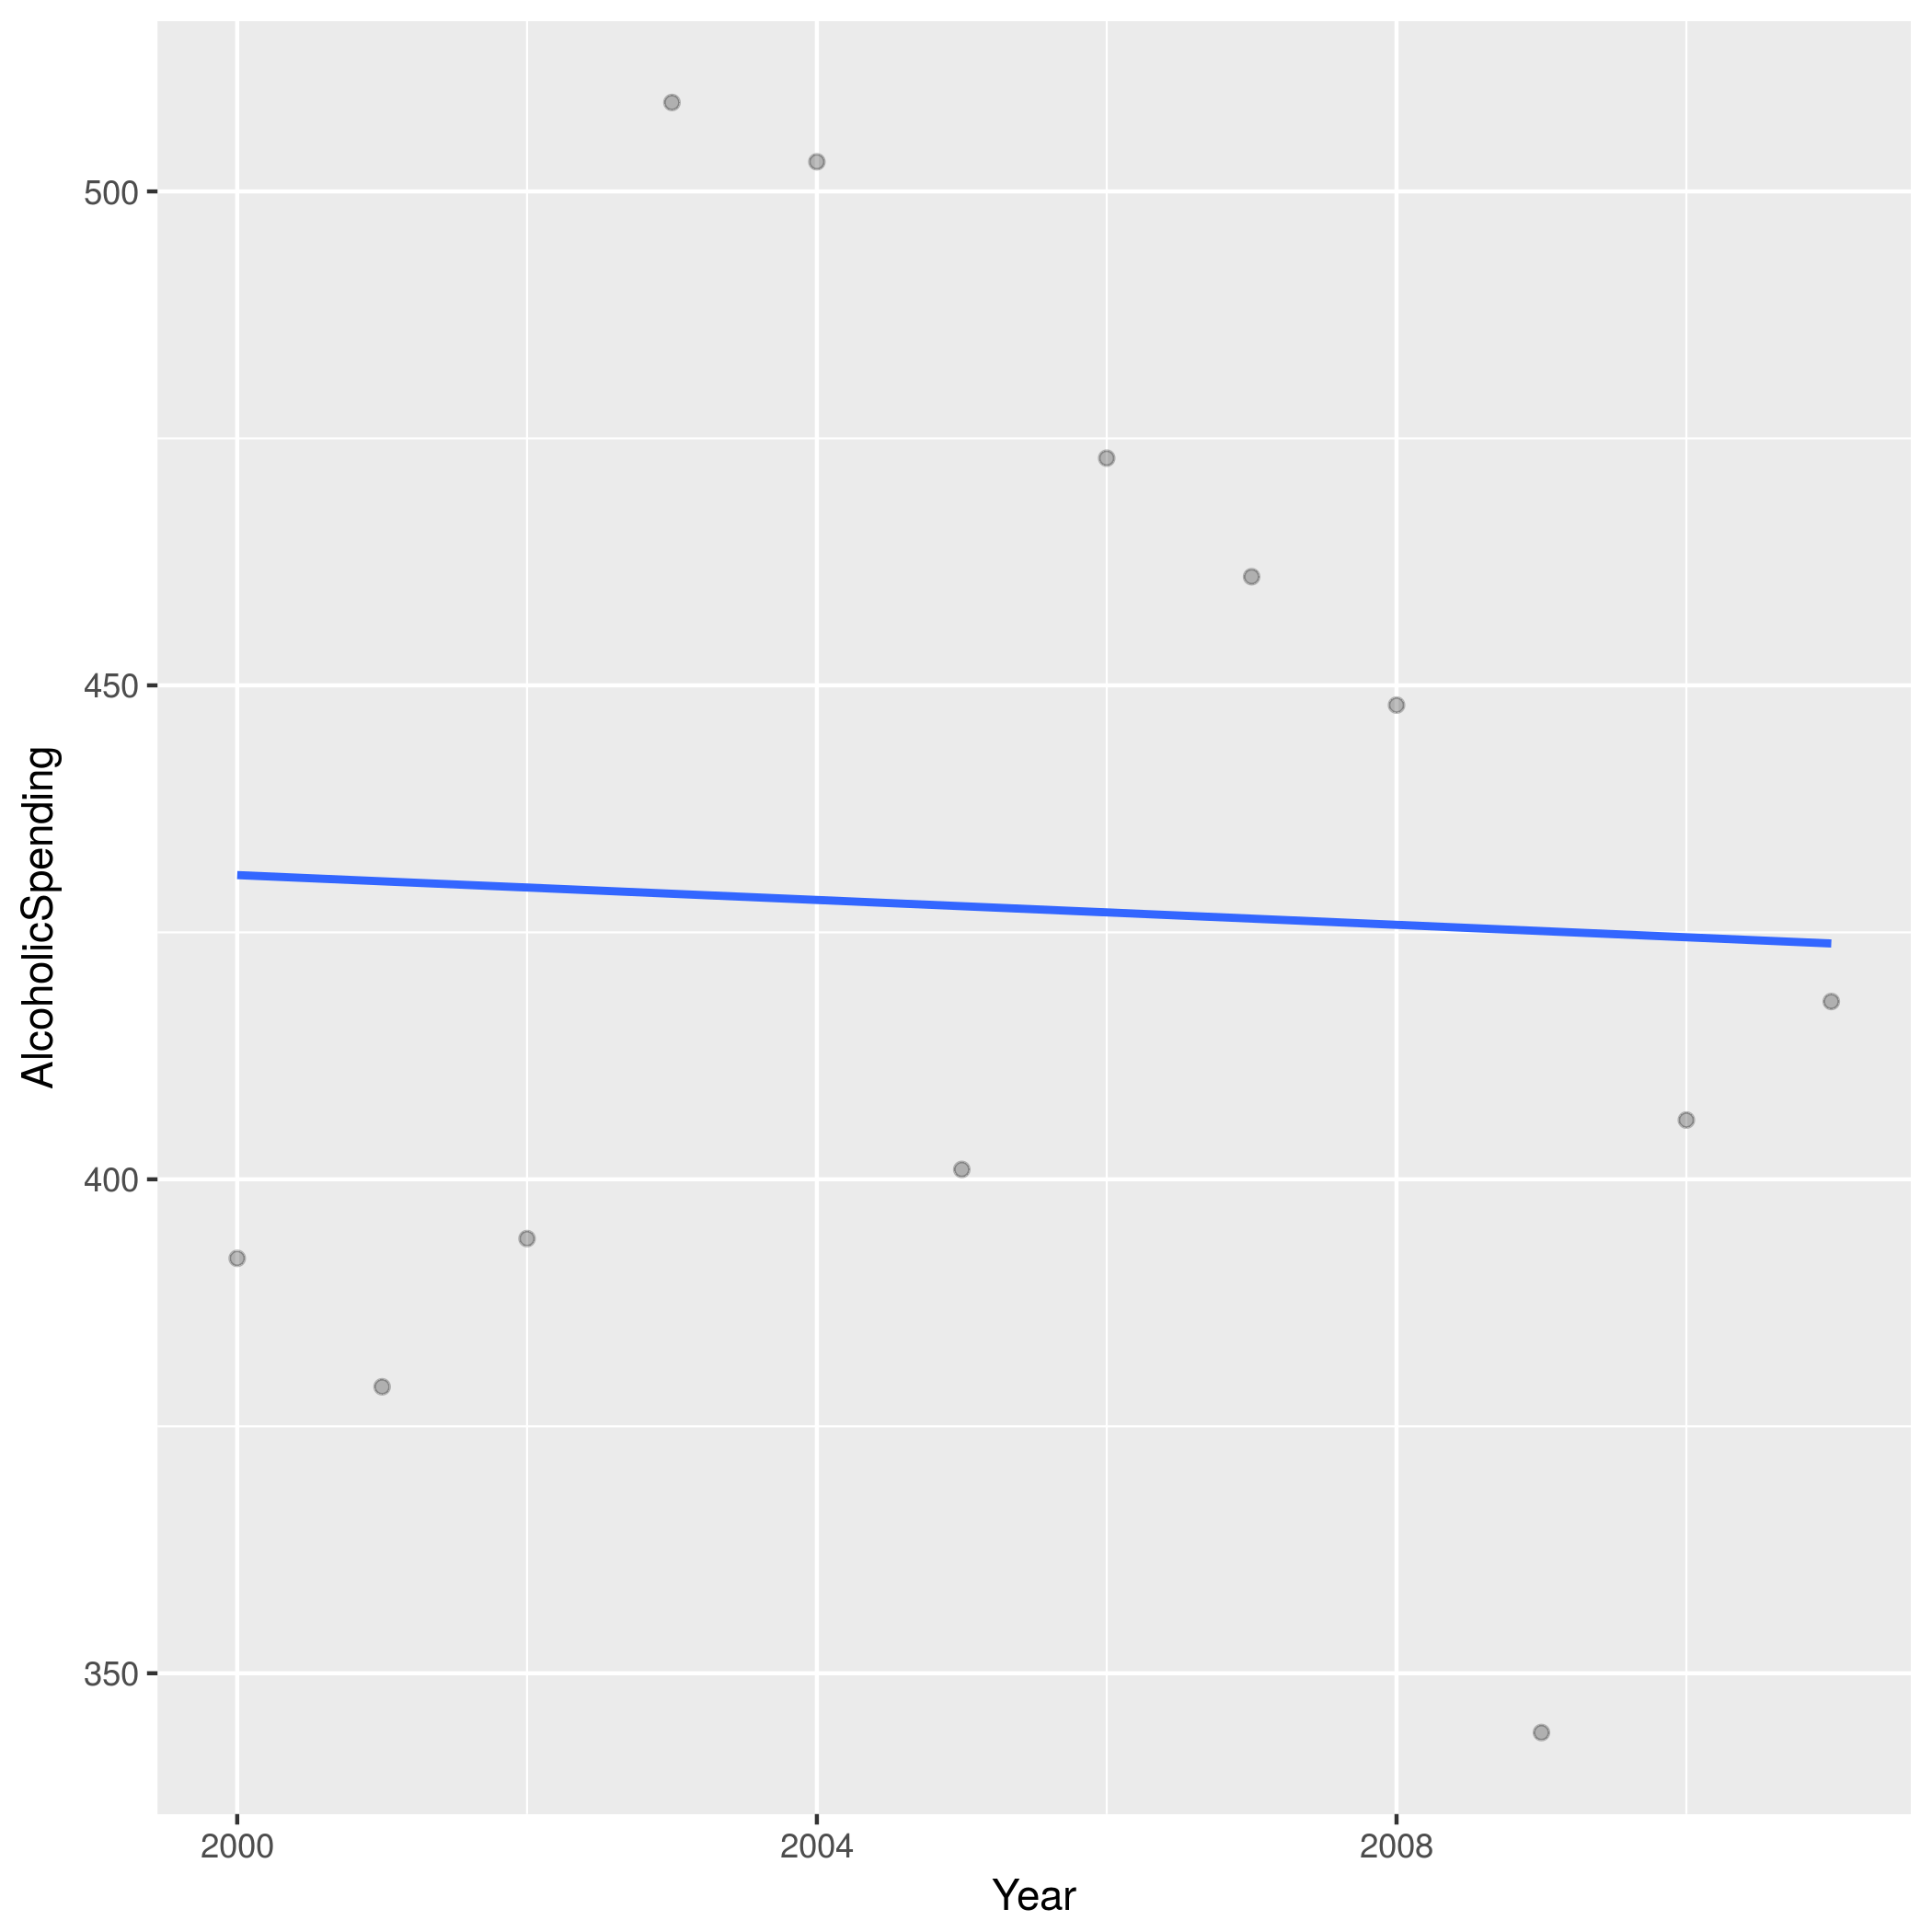
\includegraphics[widt=\textwidth]{quest1.png}
\end{figure}

\begin{figure}[h]
\caption{Health insurance among older people change throughout 10 years?}
\centering
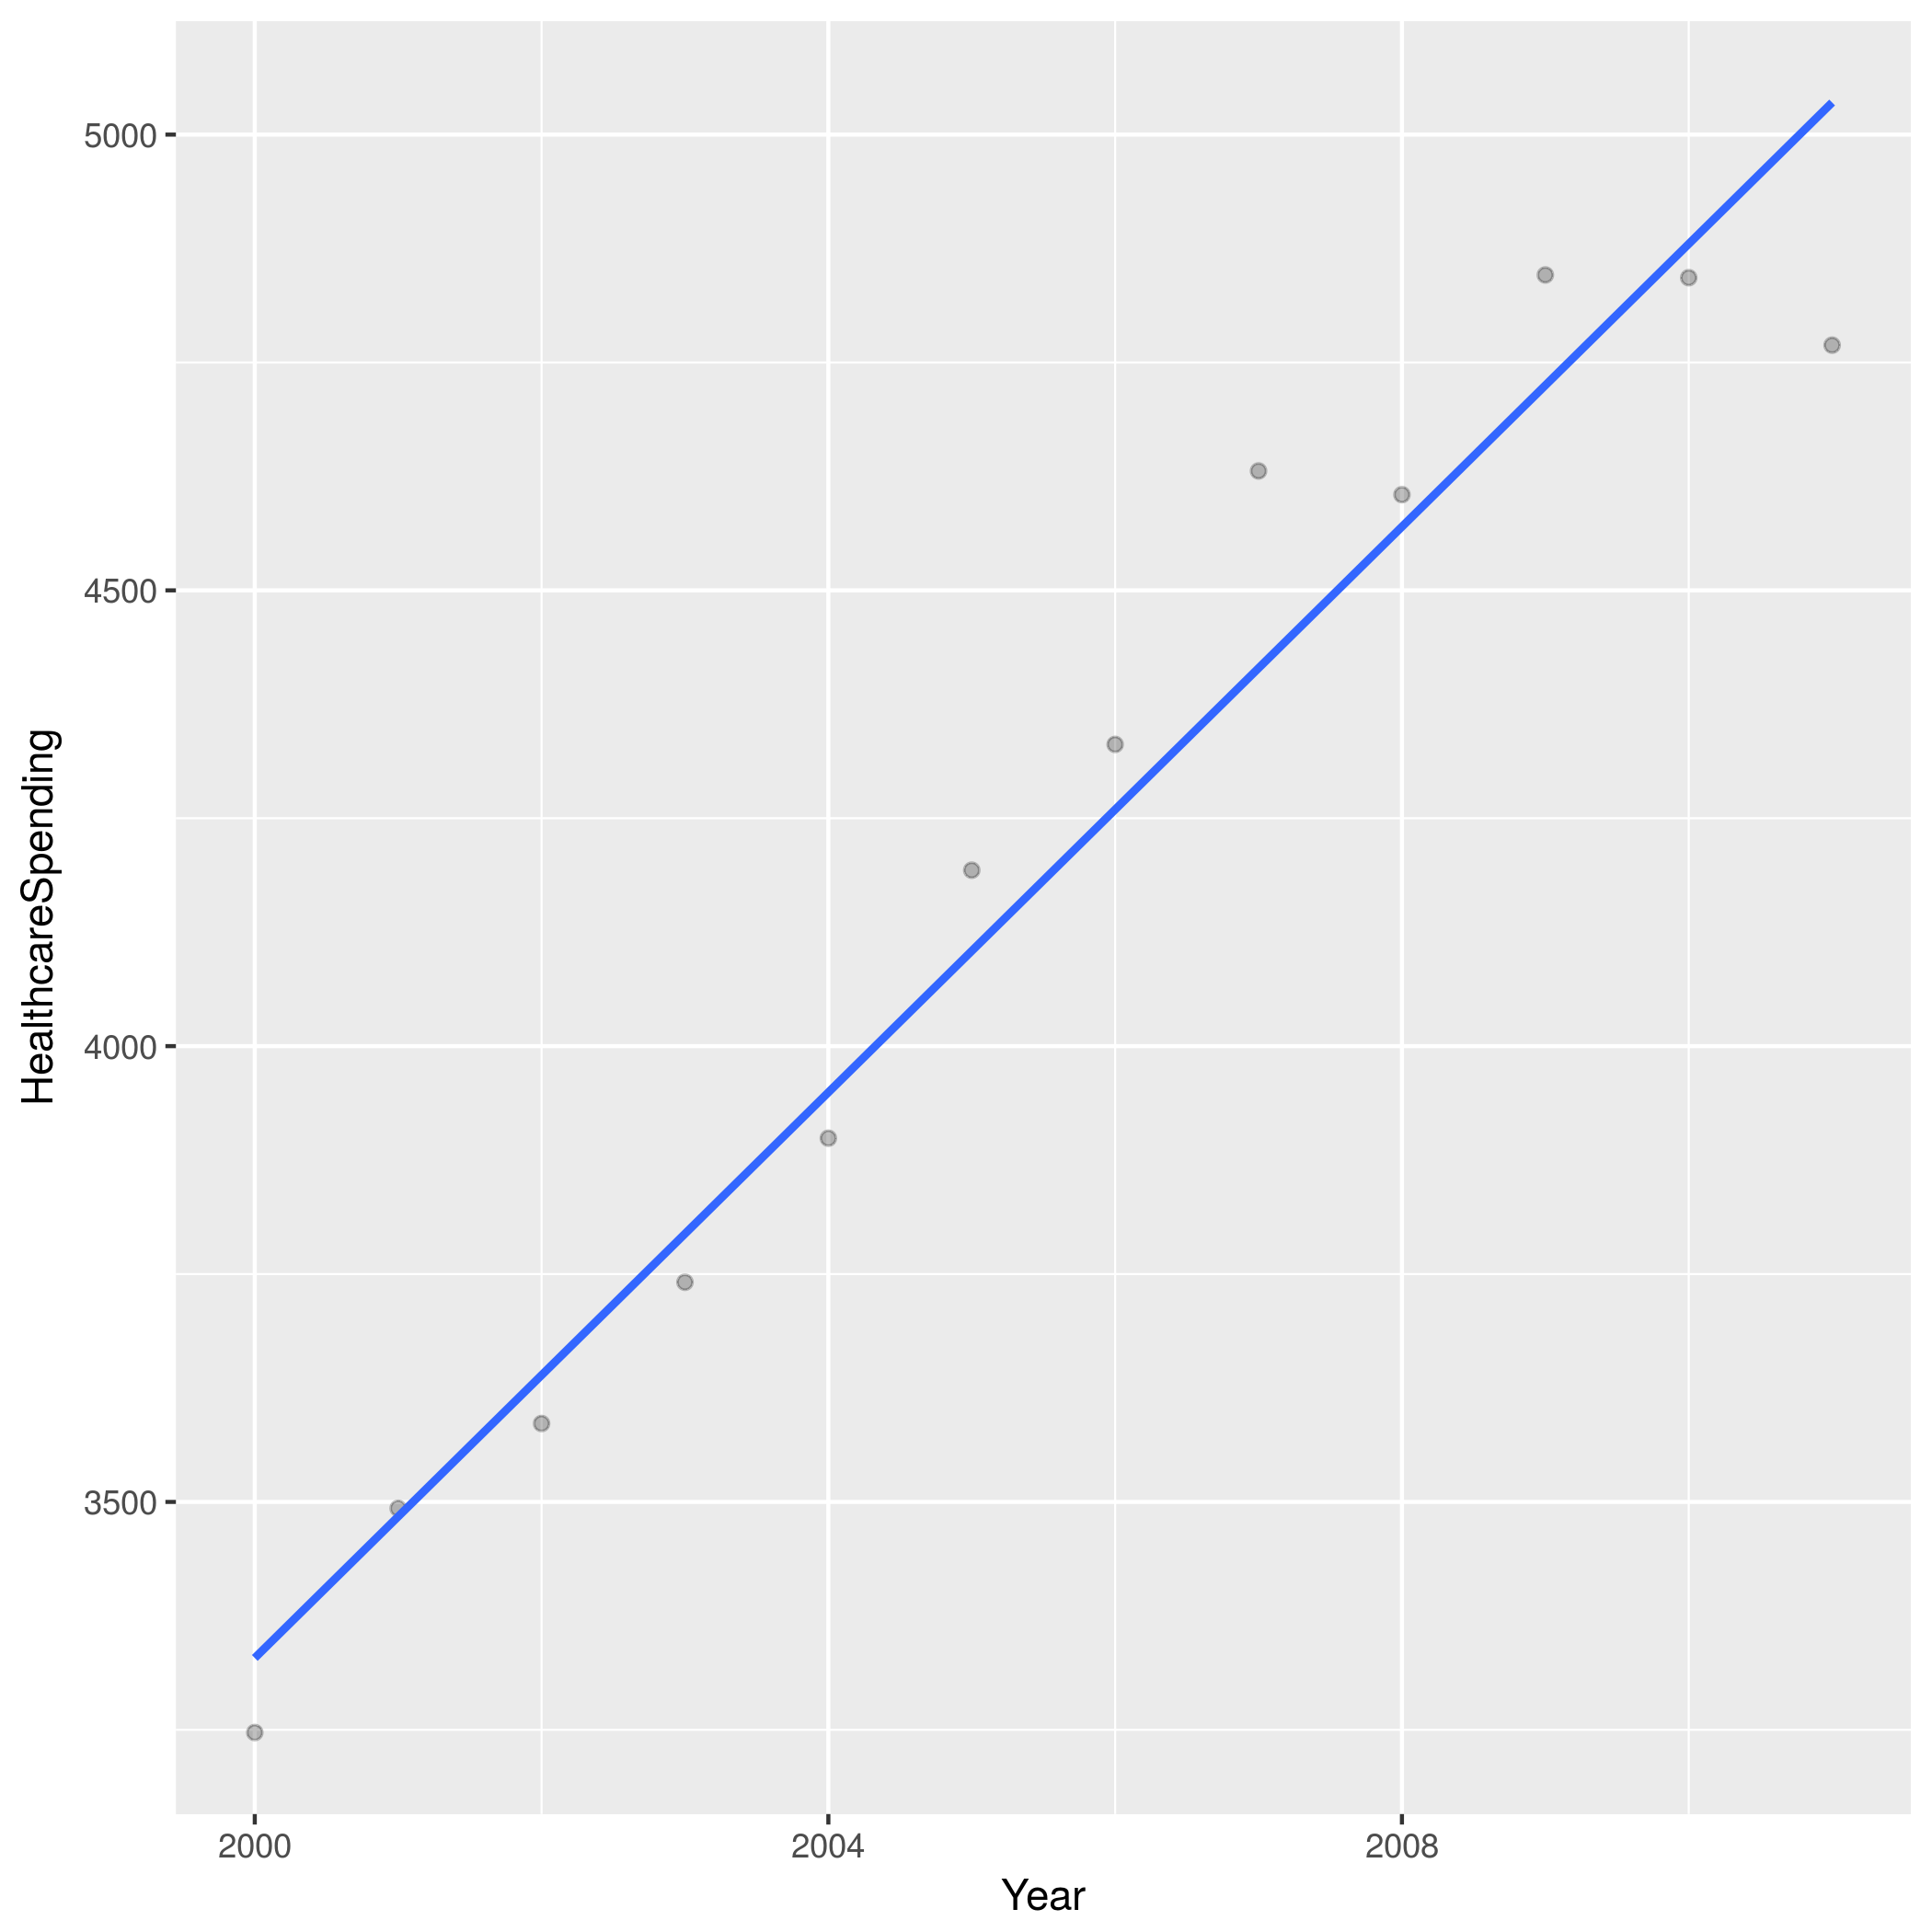
\includegraphics[widt=\textwidth]{quest2.png}
\end{figure}

\begin{figure}[h]
\caption{Health expenditure between 2000 and 2002?}
\centering
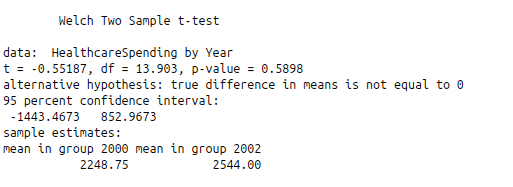
\includegraphics[widt=\textwidth]{Ttest1.png}
\end{figure}

\begin{figure}[h]
\caption{Annual expenditure between 2008 and 2009?}
\centering
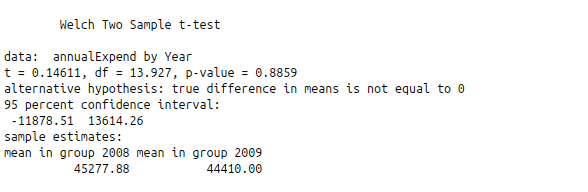
\includegraphics[widt=\textwidth]{Ttest2.png}
\end{figure}

\begin{figure}[h]
\caption{What age group spends the most amount of Money?}
\centering
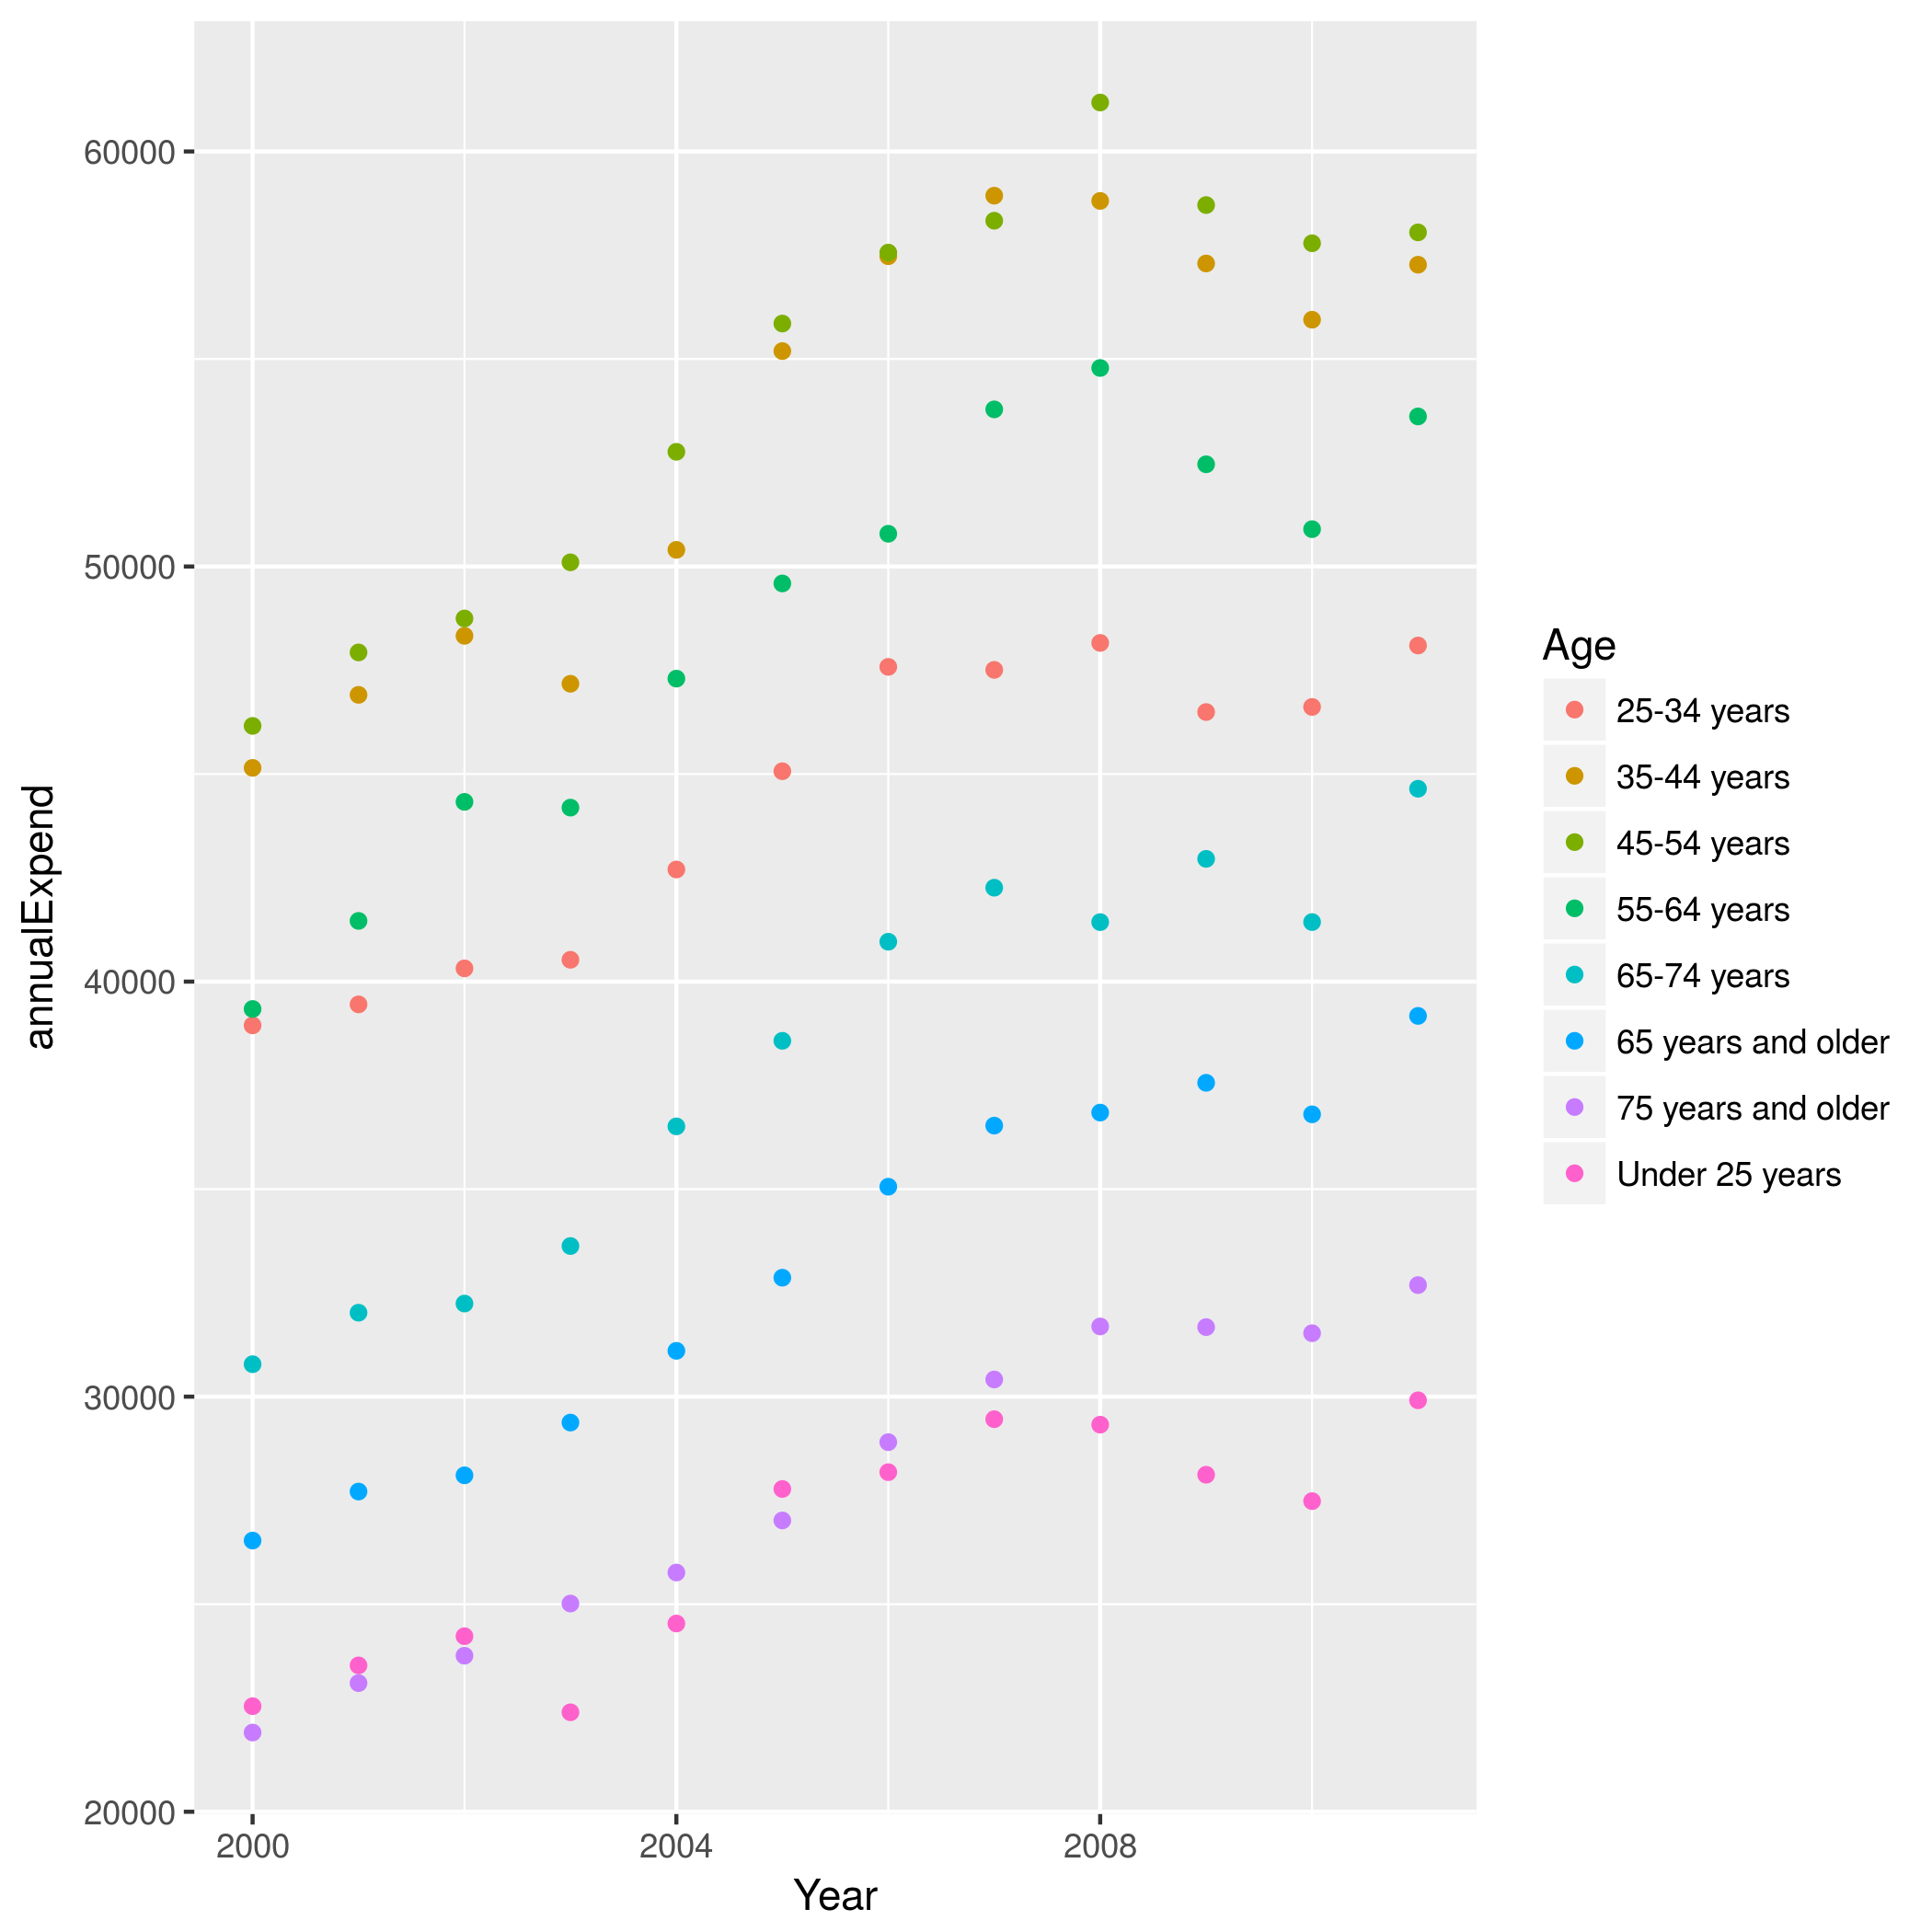
\includegraphics[widt=\textwidth]{quest5.png}
\end{figure}






\end{document}
